\documentclass{beamer}

\usepackage{parskip}
\usepackage{colortbl}
\usepackage{soul}
\usepackage{ifthen}
\usepackage[makeroom]{cancel}
\usepackage{amsthm}
\usepackage{amsmath}
\usepackage{amssymb}
\usepackage{mathtools}
\usepackage{needspace}
\usepackage{etoolbox}
\usepackage{listofitems}
\usepackage{xstring}
\usepackage{geometry}
\usepackage{tikz}
\usepackage{xcolor}
\usetikzlibrary{arrows.meta}
\usetikzlibrary{patterns}
\usetikzlibrary{external}
\usetikzlibrary{decorations.pathreplacing}
\usetikzlibrary{decorations.markings}

\usepackage{arydshln}
\setlength{\dashlinedash}{2pt}  % Finer dashes
\setlength{\dashlinegap}{2pt}     % Smaller gaps

\usetheme{boadilla}
\newcommand{\maxi}[1]{\overline{\Phi}(#1)}
\newcommand{\bir}{\text{Bir}\Diamond}
\newcommand{\ber}{\text{Ber}\Diamond}
\newcommand*\circled[1]{\tikz[baseline=(char.base)]{\node[shape=circle,draw,inner sep=1pt] (char) {#1};}}
\newcommand{\chain}[3]{#1 \stackrel{#3}{\frown} #2 }
\newcommand{\confg}{\mathcal{C}}
\newcommand{\core}{\mathcal{K}}
\newcommand{\I}{\text{I}}
\newcommand{\II}{\text{II}}
\newcommand{\compat}{\implies}
\newcommand{\ncompat}[1]{\stackrel{#1}{\compat}}
\newcommand{\digitToNum}[1]{\the\numexpr#1\relax}
\newcommand{\scheme}[2]{
    \readlist*\mylist{#2}
     \tikz[baseline]{ 
        \foreach \x [count=\i] in {#1} {
            \coordinate (\i) at (0.3*\i, 0.225); \node[text height=0mm] at (0.3*\i,0) {$\x$};
        } 
        \foreachitem \z \in \mylist {
            \StrChar{\z}{1}[\left]
            \StrChar{\z}{2}[\right]
            \StrChar{\z}{3}[\color]
            \StrChar{\z}{4}[\cross]
            \path (\left) edge[bend left=45] node[above, yshift=-2]{\small 
            \ifthenelse{\equal{\cross}{-}}{$\cancel{\color}$}{$\color$}
            } (\right);
        }
    }
} 
\definecolor{g0}{RGB}{58, 255, 36}
\definecolor{g1}{RGB}{58, 255, 36}
\definecolor{g2}{RGB}{58, 255, 36}
\definecolor{g3}{RGB}{58, 255, 36}
\definecolor{g4}{RGB}{58, 255, 36}
\definecolor{g5}{RGB}{58, 255, 36}
\definecolor{iv}{RGB}{ 255, 255, 255 }
\definecolor{rg}{RGB}{ 70, 120, 255 }
\definecolor{rb}{RGB}{ 255, 36, 36 }
\definecolor{sf}{RGB}{ 0, 0, 0 }

%Information to be included in the title page:
\title{Heart of the Four Color Theorem}
\subtitle{\small REDUCIBILITY\vspace{-0.5cm}}
\author{Timothy van der Valk\vspace{0.5cm}}
\date{}
\titlegraphic{
    \vspace{-2cm}
    \includegraphics[width=0.5\textwidth]{../paper/birkhoff_heart.pdf}
}

\AtBeginSection[]
{
  \begin{frame}
    \frametitle{Table of Contents}
    \tableofcontents[currentsection]
  \end{frame}
}

\begin{document}

\frame{\titlepage}

\newcommand{\delft}{
    \frametitle{
        \begin{minipage}{0.7\textwidth}
            Delft University of Technology     
        \end{minipage}
        \begin{minipage}{0.25\textwidth}
            \includegraphics[height=1cm]{images/logo.png}
        \end{minipage}
    }
}
\begin{frame}
    \delft
    \begin{figure}
        \includegraphics[width=0.8\textwidth]{images/campus.jpg}
    \end{figure}
\end{frame}

\begin{frame}
    \delft
    \begin{figure}
        \includegraphics[width=1\textwidth]{images/aerial.jpg}
    \end{figure}
\end{frame}

\begin{frame}
    \delft
    \begin{figure}
        \includegraphics[width=0.9\textwidth]{images/beekje.jpg}
    \end{figure}
\end{frame}

\begin{frame}
    \delft
    \begin{figure}
        \includegraphics[width=0.9\textwidth]{images/echo.jpg}
    \end{figure}
\end{frame}

\begin{frame}
    \delft
    \begin{figure}
        \includegraphics[width=0.9\textwidth]{images/library.jpg}
    \end{figure}
\end{frame}

\begin{frame}
    \delft
    \begin{figure}
        \includegraphics[width=0.9\textwidth]{images/books.jpg}
    \end{figure}
\end{frame}

\begin{frame}
    \delft
    \begin{figure}
        \includegraphics[width=0.9\textwidth]{images/delft-city.jpg}
    \end{figure}
\end{frame}

\begin{frame}
    \delft
    \begin{figure}
        \includegraphics[width=0.9\textwidth]{images/duwo.jpg}
    \end{figure}
\end{frame}

\begin{frame}
    \delft
    \begin{figure}
        \includegraphics[width=0.9\textwidth]{images/lepub.jpg}
    \end{figure}
\end{frame}

\begin{frame}
    \delft
    \begin{figure}
        \centering
        \begin{tikzpicture}
            \node at (0,0) {\includegraphics[width=0.9\textwidth]{images/aerial.jpg}};
            \node at (-3.7,-1.5) {\includegraphics[width=0.3\textwidth]{images/qrcode.png }};
        \end{tikzpicture}
        \small https://www.tudelft.nl/onderwijs/toelating-en-aanmelding/exchange-students
    \end{figure}
\end{frame}





\begin{frame}
\frametitle{Contents}
\tableofcontents
\end{frame}

\section{Part 1}

The four color theorem was initially formulated from a problem in coloring world maps. A map consists of regions that can border other regions on a flat surface. When we talk about a \textit{coloring} of a map, we mean a way to color its regions such that any two neighbors are colored differently.

The actual shape of the regions in our map is not of importance here. The key information that is needed from a map, is the connectivity between regions. Such information can be represented in a \textit{graph} where vertices (circles) correspond to regions. An edge between two vertices then indicates that the two corresponding regions are neighbors.

\begin{figure}[!h]
    \centering
    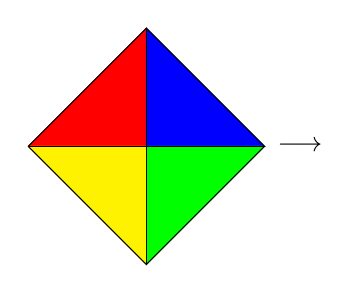
\begin{tikzpicture}[scale=1.5]
        \coordinate (v1) at (-1, 0);
        \coordinate (v2) at (0, 1);
        \coordinate (v3) at (1, 0);
        \coordinate (v4) at (0, -1);
        \coordinate (c) at (0, 0);

        \draw [fill, red] (v1) -- (v2) -- (c) -- (v1);
        \draw [fill, blue] (v2) -- (v3) -- (c) -- (v2);
        \draw [fill, green] (v3) -- (v4) -- (c) -- (v3);
        \draw [fill, yellow] (v4) -- (v1) -- (c) -- (v4);
        \draw (v1) -- (v2) -- (v3) -- (v4) -- (v1);
        \draw (c) -- (v1);
        \draw (c) -- (v2);
        \draw (c) -- (v3);
        \draw (c) -- (v4);
        \node at (1.3, 0) { $\longrightarrow$ };
    \end{tikzpicture} 
    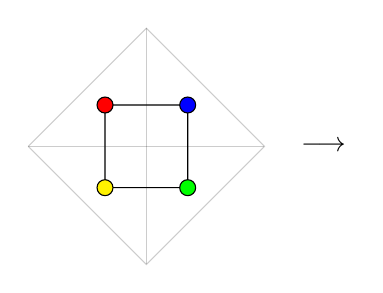
\begin{tikzpicture}[scale=1.5]
        \coordinate (v1) at (-1, 0);
        \coordinate (v2) at (0, 1);
        \coordinate (v3) at (1, 0);
        \coordinate (v4) at (0, -1);
        \coordinate (c) at (0, 0);

        \node[circle, fill, scale=0.01cm, red, draw=black] (m1) at (-0.35, 0.35) { $v_1$ };
        \node[circle, fill, scale=0.01cm, blue, draw=black] (m2) at (0.35, 0.35) { $v_2$ };
        \node[circle, fill, scale=0.01cm, green, draw=black] (m3) at (0.35, -0.35) { $v_3$ };
        \node[circle, fill, scale=0.01cm, yellow, draw=black] (m4) at (-0.35, -0.35) { $v_4$ };

        \draw (m1) -- (m2) -- (m3) -- (m4) -- (m1);
        \draw[opacity=0.2] (v1) -- (v2) -- (v3) -- (v4) -- (v1);
        \draw[opacity=0.2] (c) -- (v1);
        \draw[opacity=0.2] (c) -- (v2);
        \draw[opacity=0.2] (c) -- (v3);
        \draw[opacity=0.2] (c) -- (v4);
        \node at (1.5, 0) { $\longrightarrow$ };
    \end{tikzpicture}  
    \begin{tikzpicture}[scale=1.5, mid arrow/.style={
        postaction={ decorate, decoration={ markings, mark=at position 0.6 with { \arrow[black]{>>} } } } }]
        \coordinate (v1) at (-1, 0);
        \coordinate (v2) at (0, 1);
        \coordinate (v3) at (1, 0);
        \coordinate (v4) at (0, -1);
        \coordinate (c) at (0, 0);

        \node[circle, fill, scale=0.015cm, label=above left:$a$] (m1) at (-0.35, 0.35) { };
        \node[circle, fill, scale=0.015cm, label=above right:$b$] (m2) at (0.35, 0.35) { };
        \node[circle, fill, scale=0.015cm, label=below right:$c$] (m3) at (0.35, -0.35) { };
        \node[circle, fill, scale=0.015cm, label=below left:$d$] (m4) at (-0.35, -0.35) { };

        \draw[mid arrow] (m1) -- (m2);
        \draw (m2) -- (m3) -- (m4) -- (m1);
        \draw[opacity=0.0] (v1) -- (v2) -- (v3) -- (v4) -- (v1);
    \end{tikzpicture}      
    \caption{The translation of a map coloring to a graph coloring. In the last step we replace colors by the letters $a$,$b$,$c$ and $d$ for convenience. We obtain the coloring called $abcd$ on a \textit{planar graph}. }
    \label{fig:colortut}
\end{figure}

We will be working exclusively with \textit{planar graphs}. See Figure \ref{fig:planartut} for examples. The order of colors such as in $abcd$ is indicated by the $\gg$ edge, which is the first edge between the first two vertices. Two colorings are considered \textit{equal} if they differ only by a renaming of colors.

\begin{definition}
    A graph is \emph{planar} if it has a \emph{planar embedding} where no two edges cross each other.
\end{definition}
\begin{definition}
    \label{def:coleq}
    Two colorings $x$ and $y$ are \emph{equal} if they differ only by a renaming of the colors $a,b,c$ and $d$. I.e $abab = acac$.
\end{definition}

\begin{theorem}
    Every planar graph can be colored in at most four colors.
\end{theorem}

\begin{figure}
    \centering
    \begin{tikzpicture}[scale=1.5]
        \coordinate (v1) at (-1, 0);
        \coordinate (v2) at (0, 1);
        \coordinate (v3) at (1, 0);
        \coordinate (v4) at (0, -1);
        \coordinate (c) at (0, 0);

        \node[circle, fill, scale=0.015cm] (m1) at (-0.35, 0.35) { };
        \node[circle, fill, scale=0.015cm] (m2) at (0.35, 0.35) { };
        \node[circle, fill, scale=0.015cm] (m3) at (0.35, -0.35) { };
        \node[circle, fill, scale=0.015cm] (m4) at (-0.35, -0.35) { };

        \draw (m1) -- (m2);
        \draw (m2) -- (m3) -- (m4) -- (m1);
        \draw (m1) -- (m3);
        \draw (m2) -- (m4);
        \draw[opacity=0.0] (v1) -- (v2) -- (v3) -- (v4) -- (v1);
    \end{tikzpicture}
    \begin{tikzpicture}[scale=1.5]
        \coordinate (v1) at (-1, 0);
        \coordinate (v2) at (0, 1);
        \coordinate (v3) at (1, 0);
        \coordinate (v4) at (0, -1);
        \coordinate (c) at (0, 0);

        \node[circle, fill, scale=0.015cm] (m1) at (-0.35, 0.35) { };
        \node[circle, fill, scale=0.015cm] (m2) at (0.35, 0.35) { };
        \node[circle, fill, scale=0.015cm] (m3) at (0.35, -0.35) { };
        \node[circle, fill, scale=0.015cm] (m4) at (-0.35, -0.35) { };

        \draw (m2) -- (m4);
        \draw (m1) .. controls +(0.7, 0.7) and +(0.7, 0.7) .. (m3);
        \draw (m1) -- (m2);
        \draw (m2) -- (m3) -- (m4) -- (m1);
        \draw[opacity=0.0] (v1) -- (v2) -- (v3) -- (v4) -- (v1);
    \end{tikzpicture}
    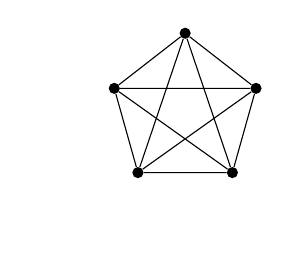
\begin{tikzpicture}
        \node[circle, fill, scale=0.015cm] (l1) at (0, 1) { };
        \node[circle, fill, scale=0.015cm] (l2) at (0.9, 0.30) { };
        \node[circle, fill, scale=0.015cm] (l3) at (0.6, -0.77) {};
        \node[circle, fill, scale=0.015cm] (l4) at (-0.6, -0.77) {};
        \node[circle, fill, scale=0.015cm] (l5) at (-0.9, 0.30) {};
        \node[circle, fill, scale=0cm] at (-2, -1.5) {};

        \draw (l1) -- (l3) -- (l5) -- (l2) -- (l4) -- (l1);
        \draw (l1) -- (l2) -- (l3) -- (l4) -- (l5) -- (l1);
        
    \end{tikzpicture}
    \caption{A non-planar embedding of the full graph $K_4$ on 4 vertices (left). A planar embedding of $K_4$ (middle), therefore $K_4$ is a planar graph. A non-planar graph $K_5$ that has no planar embeddings (right). }
    \label{fig:planartut}
\end{figure}
\subsection{Rings}
\label{subsec:rings}

We have seen in the proof of the five color theorem that a vertex surrounded by five or less neighbors can always be colored using one of five colors, even if all of its neighbors initially use all five colors. If we have only four colors available, we will find that it is no longer guaranteed that we can free a color. This is what Alfred Kempe tried to do when he gave the first false proof of the four color theorem.

If we look at the key idea, we see that if one half of a graph is isolated from another half by a group of boundary vertices, we can color this isolated part regardless of the colors on the boundary. Naturally, the fundamental shape that seperates a graph in two halves is a \textit{ring} (or a line if it is not cyclic).

\begin{definition}
    A \emph{ring} of $n$ vertices $R_n$ in a planar graph $G$ is an induced cycle of $G$.
\end{definition}

An example of what is a ring and what is not can be seen in Figure \ref{fig:ring}.

\begin{figure}[!ht]
    \centering
    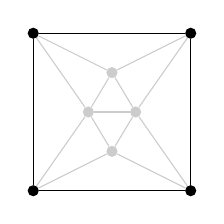
\begin{tikzpicture}
        \node[circle, fill, scale=0.015cm] (l1) at (-1, -1) { };
            \node[circle, fill, scale=0.015cm] (l2) at (-1, 1) { };
            \node[circle, fill, scale=0.015cm] (l3) at (1, 1) {};
            \node[circle, fill, scale=0.015cm] (l4) at (1, -1) {};
            \node[circle, fill, scale=0.015cm, opacity=0.2] (m1) at (0, 0.5) {};
            \node[circle, fill, scale=0.015cm, opacity=0.2] (m2) at (-0.3, 0) {};
            \node[circle, fill, scale=0.015cm, opacity=0.2] (m3) at (0.3, 0) {};
            \node[circle, fill, scale=0.015cm, opacity=0.2] (m4) at (0, -0.5) {};

            \draw (l1) -- (l2) -- (l3) -- (l4) -- (l1);
            \draw[opacity=0.2] (m1) -- (m2) -- (m4) -- (m3) -- (m1);
            \draw[opacity=0.2] (m2) -- (m3);
            \draw[opacity=0.2] (m1) -- (l2);
            \draw[opacity=0.2] (m1) -- (l3);
            \draw[opacity=0.2] (m2) -- (l1);
            \draw[opacity=0.2] (m2) -- (l2);
            \draw[opacity=0.2] (m3) -- (l3);
            \draw[opacity=0.2] (m3) -- (l4);
            \draw[opacity=0.2] (m4) -- (l1);
            \draw[opacity=0.2] (m4) -- (l4);
    \end{tikzpicture}
    \hspace{1cm}
    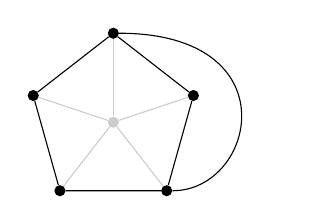
\begin{tikzpicture}[scale=1.13]
        \node[circle, fill, scale=0.015cm, opacity=0.2] (c) at (0, 0) {};


        \node[circle, fill, scale=0.015cm] (l1) at (0, 1) { };
        \node[circle, fill, scale=0.015cm] (l2) at (0.9, 0.30) { };
        \node[circle, fill, scale=0.015cm] (l3) at (0.6, -0.77) {};
        \node[circle, fill, scale=0.015cm] (l4) at (-0.6, -0.77) {};
        \node[circle, fill, scale=0.015cm] (l5) at (-0.9, 0.30) {};

        \draw[opacity=0.2] (c) -- (l1);
        \draw[opacity=0.2] (c) -- (l2);
        \draw[opacity=0.2] (c) -- (l3);
        \draw[opacity=0.2] (c) -- (l4);
        \draw[opacity=0.2] (c) -- (l5);
        \draw (l1) -- (l2) -- (l3) -- (l4) -- (l5) -- (l1);
        \draw (l1) .. controls +(2,0) and +(1,0) .. (l3);
    \end{tikzpicture}
    \caption{In bold, an example of the ring $R_4$ surrounding a graph on four vertices (left) and an example of an invalid ring $R_5$. No extra edges are allowed between ring vertices, since otherwise the ring is not an induced cycle of $G$. }
    \label{fig:ring}
\end{figure}

We will frequently need all the possible colorings for a ring $R$ contained in a certain planar graph $G$. Let us give a name to the set of such colorings.

\begin{definition}
    The set of all 4-colorings of a ring $R$ in a planar graph $G$ is given by $\Phi(R \subset G)$ or $\Phi(G)$ if $R$ is clear from the context. We let $\Phi(n) = \Phi(R_n)$, the set of all possible ring colorings of $R_n$.
\end{definition}

The first thing we might do with rings is see if they themselves are reducible. In fact, we will find a common result from literature.

\begin{theorem}
    \label{thm:ringsarered}
    The ring $R_n$ with $n\geq 4$ is reducible in every planar graph $G$.
\end{theorem}

\begin{proof}
Let $R_n$ be strongly-contained in $G$. Since the interior of $R_n$ is empty and $n\geq4$, we may contract any two non-neighboring ring vertices $u$ and $v$ to a new vertex $y$. As a result, we obtain the graph $G'$ on one less vertex. 

Given a 4-coloring of $G'$. Because $R_n$ is a ring, there will be no edges between the ring vertices $u$ and $v$. Therefore, we may give $u$ and $v$ the same color as $y$ without issue. Let the other vertices of $G$ be given the same color as their $G'$ counterparts. Then we have obtained a 4-coloring of $G$.

\end{proof}

\begin{figure}[!ht]
    \centering
    \begin{tikzpicture}[scale=0.7]
        \node (l1) at (-1, -1) { $a$ };
        \node (l2) at (-1, 1) { $b$ };
        \node (l3) at (1, 1) { $c$ };
        \node (l4) at (1, -1) { $b$ };

        \draw (l1) -- (l2) -- (l3) -- (l4) -- (l1);
        \node (impl) at (2.3, 0) { $\Longleftrightarrow$ };
        \draw[dotted, thick] (l2) -- (l4);
    \end{tikzpicture}
    \begin{tikzpicture}[scale=0.7]
        \node (l1) at (-1, -1) { $a$ };
        \node[opacity=0.2] (l2) at (-1, 1) { $b$ };
        \node (l3) at (1, 1) { $c$ };
        \node[opacity=0.2] (l4) at (1, -1) { $b$ };
        \node (c) at (0, 0) { $b$ };

        \draw (l1) -- (c) -- (l3);
        \draw[dotted, thick, opacity=0.2] (l2) -- (c) -- (l4);
    \end{tikzpicture}
    \caption{The ring $R_4$ being contracted to a smaller graph $G'$. The coloring of $G'$ can be reversed to a coloring of $G$.}
\end{figure}

In the next section we will be treating the reducibility of configurations with a ring as their boundary. It might not be a surprise then that the reducibility of plain rings is a key ingredient in the reducibility of these configurations, too. In Section \ref{sec:creduce} we will see that this form of reducibility with contractions is actually C-reducibility. Therefore, in the context of Theorem \ref{funda1}, plain rings can be considered as C-reducible configurations. 
\begin{frame}
    \includegraphics[width=\textwidth]{images/break1.png}
    We will be back in 5 minutes.
\end{frame}

\section{Part 2}
\subsection{0-reducibility of the ring $R_4$}

We will show that all configurations on the ring $R_4$ are reducible without the need for a reducer. This proof and the proof of the five color theorem are very much alike.

\begin{theorem}
    The ring $R_4$ is 0-reducible.
\end{theorem}
\begin{proof}

Let the planar graph $M+\confg$ with configuration $\confg = \core + R_4$ be arbitrary. Since we set $k=0$, we will try reducing to $M+R_4$ and $\confg$. For convenience, let the possible ring colorings of these two reductions be represented by the sets

\begin{equation}
    \I = \Phi(M+R_4) \quad \text{and} \quad \II = \Phi(\confg).
\end{equation}

To gain an insight into the possible colorings of these sets, we sketched the situation in Figure \ref{fig:ring4tut}.

\begin{figure}[!ht]
    \centering
    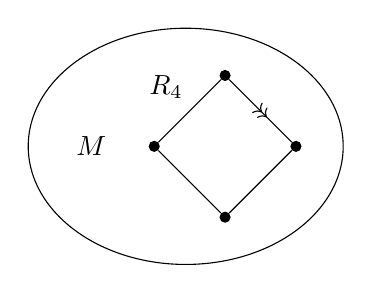
\begin{tikzpicture}[mid arrow/.style={
        postaction={ decorate, decoration={ markings, mark=at position 0.6 with { \arrow[black]{>>} } } } }]
        \draw[fill=white] (-0.5, 0) ellipse (2cm and 1.5cm);
        \node (m) at (-1.7, 0) {$M$};
        \node at (-0.75, 0.75) {$R_4$};

        \node[circle, fill, scale=0.015cm] (l1) at (0, 0.9) { };
        \node[circle, fill, scale=0.015cm] (l2) at (0.9, 0) { };
        \node[circle, fill, scale=0.015cm] (l3) at (0, -0.9) {};
        \node[circle, fill, scale=0.015cm] (l4) at (-0.9, 0) {};

        \draw[mid arrow] (l1) -- (l2);
        \draw (l2) -- (l3) -- (l4) -- (l1);
    \end{tikzpicture}
    \begin{tikzpicture}[mid arrow/.style={
        postaction={ decorate, decoration={ markings, mark=at position 0.6 with { \arrow[black]{>>} } } } }]
        \draw[opacity=0] (-0.5, 0) ellipse (2cm and 1.5cm);
        \node at (-0.75, 0.75) {$R_4$};
        \node[inner sep=1mm] (c) at (0, 0) {$\core$};

        \node[circle, fill, scale=0.015cm] (l1) at (0, 0.9) { };
        \node[circle, fill, scale=0.015cm] (l2) at (0.9, 0) { };
        \node[circle, fill, scale=0.015cm] (l3) at (0, -0.9) {};
        \node[circle, fill, scale=0.015cm] (l4) at (-0.9, 0) {};

        \draw[mid arrow] (l1) -- (l2);
        \draw (l2) -- (l3) -- (l4) -- (l1);
        \draw[opacity=0.2] (l1) -- (c);
        \draw[opacity=0.2] (l2) -- (c); 
        \draw[opacity=0.2] (l3) -- (c);
        \draw[opacity=0.2] (l4) -- (c);
    \end{tikzpicture}
    \caption{The reductions $M+R_4$ and $\core+R_4$ ($\confg$). What can we say about their possible ring colorings $\I$ and $\II$?}
    \label{fig:ring4tut}
\end{figure}

You might have noticed that both reductions contain the plain ring $R_4$ with no other vertices on one side. Therefore, as we have shown in Theorem \ref{thm:ringsarered} about plain ring reducibility, we may contract any two non-neighboring vertices to obtain further reductions.

We wont sketch these contracted graphs here, but in the context of ring colorings in $\I$ and $\II$, we will obtain colorings of $R_4$ with two contracted vertices colored the same. Because there are two ways to contract vertices on $R_4$ (the two diagonals), we are guaranteed of the following two colorings in $\I$ and $\II$.

\begin{equation}
    \left\{\begin{matrix}
        abab \;\;\text{or}\;\; abac, \\
        baba \;\;\text{or}\;\; baca
    \end{matrix}\right\} \subset I,II.
\end{equation}

Let us evaluate every pair of possibilities to see if there is a common coloring. First note that $abab=baba$ by definition of equality between ring colorings (Definition \ref{def:coleq}). Then, there remain 3 possible sets for $\I$ and $\II$.

\needspace{2cm}
\begin{equation}
    \circled{1} = \{ abab \}, \quad \circled{2} = \left\{ \begin{matrix}abab \\ baca\end{matrix} \right\}, \quad \circled{3} = \left\{ \begin{matrix}abac \\ baca \end{matrix} \right\}.
\end{equation}

You might already see that there is only one pair where we must actually show something, because
\begin{enumerate}
    \item $\I = \circled{1}$ and $\II = \circled{2}$ implies that $abab$ is the common coloring.
    \item $\I = \circled{2}$ and $\II = \circled{3}$ implies that $baca$ is the common coloring.
    \item $\I = \circled{1}$ and $\II = \circled{3}$. This is where Kempe-chains come in.
\end{enumerate}

To handle the third case, let $\I = \{ abab \}$ and $\II = \{ abac, baca \}$. Similar to what we did with the five color theorem, suppose that in the coloring $\I(abab)$ we have $\chain{v_1}{v_3}{ad}$. In both cases we obtain

\begin{equation}
    \begin{aligned}
        \I(abab) &= \scheme{a,b,a,b}{13d} \compat \II(abac) \\
        \I(abab) &= \scheme{a,b,a,b}{13d-} \compat \I(abcb) = \II(baca).
    \end{aligned}
\end{equation}

In any case, we obtain a common ring coloring between $\I$ and $\II$. Therefore the ring $R_4$ is 0-reducible.
\end{proof}
\subsection{1-reducibility of ring $R_5$}

\begin{frame}
    \frametitle{1-reducibility of ring $R_5$}

    \begin{theorem}<1->
        The ring $R_5$ is 1-reducible
    \end{theorem}

    \uncover<2->{
        \textit{Proof.} We will show that there is a common ring coloring for any $M+S$ and $\core + S'$.

        Let the ring colorings of the two graphs again be given by
        \begin{equation}
            \I = \Phi(M+S) \quad \text{and} \quad \II = \Phi(\core+S').
        \end{equation}

        We can choose to reduce with any $S$ and $S'$ on $\leq 1$ extra vertices. Each choice gives us guaranteed colorings for I and II.
    }
\end{frame}

\begin{frame}
    \frametitle{1-reducibility of ring $R_5$}
    First we examine the guaranteed colorings without using a reducer.

    \begin{figure}[!ht] 
        \centering
        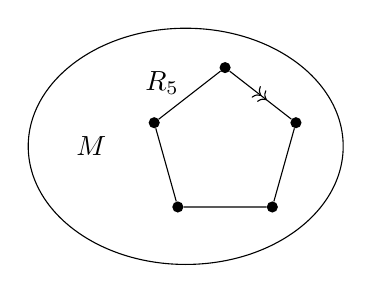
\begin{tikzpicture}[mid arrow/.style={
            postaction={ decorate, decoration={ markings, mark=at position 0.6 with { \arrow[black]{>>} } } } }]
            \draw[fill=white] (-0.5, 0) ellipse (2cm and 1.5cm);
            \node (m) at (-1.7, 0) {$M$};
            \node at (-0.8, 0.8) {$R_5$};
    
            \node[circle, fill, scale=0.015cm] (l1) at (0, 1) { };
            \node[circle, fill, scale=0.015cm] (l2) at (0.9, 0.30) { };
            \node[circle, fill, scale=0.015cm] (l3) at (0.6, -0.77) {};
            \node[circle, fill, scale=0.015cm] (l4) at (-0.6, -0.77) {};
            \node[circle, fill, scale=0.015cm] (l5) at (-0.9, 0.30) {};
            \draw[mid arrow] (l1) -- (l2);
            \draw (l2) -- (l3) -- (l4) -- (l5) -- (l1);
        \end{tikzpicture}
        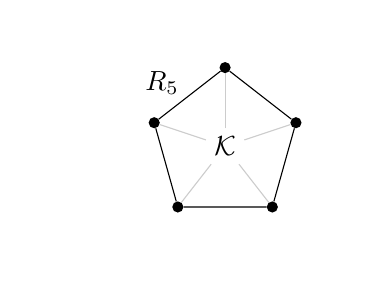
\begin{tikzpicture}[mid arrow/.style={
            postaction={ decorate, decoration={ markings, mark=at position 0.6 with { \arrow[black]{>>} } } } }]
            \draw[opacity=0] (-0.5, 0) ellipse (2cm and 1.5cm);
            \node at (-0.8, 0.8) {$R_5$};
            \node[inner sep=1mm] (c) at (0, 0) {$\core$};
            \node[circle, fill, scale=0.015cm] (l1) at (0, 1) { };
            \node[circle, fill, scale=0.015cm] (l2) at (0.9, 0.30) { };
            \node[circle, fill, scale=0.015cm] (l3) at (0.6, -0.77) {};
            \node[circle, fill, scale=0.015cm] (l4) at (-0.6, -0.77) {};
            \node[circle, fill, scale=0.015cm] (l5) at (-0.9, 0.30) {};
    
            \draw[opacity=0.2] (c) -- (l1);
            \draw[opacity=0.2] (c) -- (l2);
            \draw[opacity=0.2] (c) -- (l3);
            \draw[opacity=0.2] (c) -- (l4);
            \draw[opacity=0.2] (c) -- (l5);
            \draw (l1) -- (l2) -- (l3) -- (l4) -- (l5) -- (l1);
        \end{tikzpicture}
        \caption{The reductions $M+R_5$ and $\core+R_5$.}
        \label{fig:ring5k0}
    \end{figure}

    These plain rings $R_5$ in each graph may be further reduced by contracting two opposing vertices.
    
\end{frame}

\begin{frame}
    \frametitle{1-reducibility of ring $R_5$}
    
    We can contract two opposing vertices of $R_5$ in 5 different ways. Each choice guarantees a coloring where two vertices are colored the same.

    \uncover<2->{
    \begin{equation}
        \Phi^\star = \{ a{*}{*}a{*}, \quad {*}a{*}{*}a, \quad a{*}a{*}{*}, \quad {*}a{*}a{*}, \quad {*}{*}a{*}a{*} \}.
    \end{equation}
    }

    \uncover<3->{
        The ${*}$-colors are still unknown, but we are guaranteed that the colorings are possible, therefore $\Phi^\star \subset \I,\II$.
    }
\end{frame}

\begin{frame}
    \frametitle{1-reducibility of ring $R_5$}

    Next, we examine the guaranteed colorings with a reducer that has 1 extra vertex.

    \uncover<2->{\begin{figure}[!ht]
    \centering
    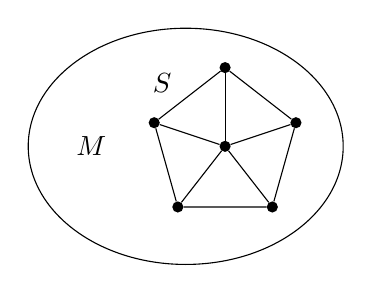
\begin{tikzpicture}[mid arrow/.style={
        postaction={ decorate, decoration={ markings, mark=at position 0.6 with { \arrow[black]{>>} } } } }]
        \draw[fill=white] (-0.5, 0) ellipse (2cm and 1.5cm);
        \node (m) at (-1.7, 0) {$M$};
        \node at (-0.8, 0.8) {$S$};

        \node[circle, fill, scale=0.015cm] (l1) at (0, 1) { };
        \node[circle, fill, scale=0.015cm] (l2) at (0.9, 0.30) { };
        \node[circle, fill, scale=0.015cm] (l3) at (0.6, -0.77) {};
        \node[circle, fill, scale=0.015cm] (l4) at (-0.6, -0.77) {};
        \node[circle, fill, scale=0.015cm] (l5) at (-0.9, 0.30) {};
        \node[circle, fill, scale=0.015cm] (e) at (0, 0) { };

        \draw (e) -- (l1);
        \draw (e) -- (l2);
        \draw (e) -- (l3);
        \draw (e) -- (l4);
        \draw (e) -- (l5);
        \draw (l1) -- (l2);
        \draw (l2) -- (l3) -- (l4) -- (l5) -- (l1);
    \end{tikzpicture}
    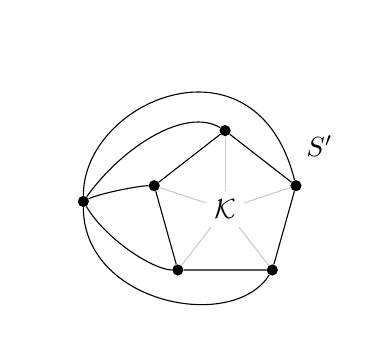
\begin{tikzpicture}[mid arrow/.style={
        postaction={ decorate, decoration={ markings, mark=at position 0.6 with { \arrow[black]{>>} } } } }]
        \draw[opacity=0] (-0.5, 0) ellipse (2cm and 1.5cm);
        \node[fill=white] at (1.2, 0.8) {$S'$};
        \node[inner sep=1mm] (c) at (0, 0) {$\core$};
        \node[circle, fill, scale=0.015cm] (l1) at (0, 1) { };
        \node[circle, fill, scale=0.015cm] (l2) at (0.9, 0.30) { };
        \node[circle, fill, scale=0.015cm] (l3) at (0.6, -0.77) {};
        \node[circle, fill, scale=0.015cm] (l4) at (-0.6, -0.77) {};
        \node[circle, fill, scale=0.015cm] (l5) at (-0.9, 0.30) {};
        \node[circle, fill, scale=0.015cm] (e) at (-1.8, 0.1) { };

        \draw (e) .. controls +(0.2, 0.1) and + (-0.2, 0.0) .. (l5);
        \draw (e) .. controls +(0.3, -0.5) and +(-0.3,0) .. (l4);
        \draw (e) .. controls +(0.0,-1.3) and +(-0.5,-0.8) .. (l3);
        \draw (e) .. controls +(0.0,+1.3) and +(-0.5,+2) .. (l2);
        \draw (e) .. controls +(0.5,0.7) and +(-0.5, 0.3) .. (l1);

        \draw[opacity=0.2] (c) -- (l1);
        \draw[opacity=0.2] (c) -- (l2);
        \draw[opacity=0.2] (c) -- (l3);
        \draw[opacity=0.2] (c) -- (l4);
        \draw[opacity=0.2] (c) -- (l5);
        \draw (l1) -- (l2) -- (l3) -- (l4) -- (l5) -- (l1);
    \end{tikzpicture}
    \caption{The reductions $M+S$ and $\core+S'$.}
\end{figure}}

    \uncover<3->{
        These reducers guarantee \textbf{one} 3-coloring of the ring.
    }
\end{frame}

\begin{frame}
    \frametitle{1-reducibility of ring $R_5$}

    These reducers guarantee \textbf{one} 3-coloring of the ring $R_5$.

    \uncover<2->{
    \begin{equation}
        \Phi^S = \{ 
            \underline{c}abab\;\;\textbf{or}\;\; 
            a\underline{c}bab\;\;\textbf{or}\;\;
            ab\underline{c}ab\;\;\textbf{or}\;\;
            aba\underline{c}b\;\;\textbf{or}\;\;
            abab\underline{c} \}.
    \end{equation}
    }

    \uncover<3->{
        In total, we are guaranteed of two sets of colorings for $\I$ and $\II$.

        \begin{equation*}
            \Phi^\star, \Phi^S \; \subset \I,\II.
        \end{equation*}

        Next, we show that these guaranteed colorings are sufficient to find a common coloring in $\I$ and $\II$.
    }
\end{frame}

\begin{frame}
    \frametitle{1-reducibility of ring $R_5$}
    The 3-colorings are important because of two key properties that they have.

    \begin{definition}<2->
        The uniquely-colored vertex of a 3-coloring of $R_5$ is called the \emph{marked vertex}, indicated by an underline such as in $\underline{c}abab$.
    \end{definition}
    
    \begin{definition}<3->
        Two 3-colorings of $R_5$ are called \emph{adjacent} if they have adjacent marked vertices, such as in $\underline{c}abab$ and $a\underline{c}bab$.
    \end{definition}
\end{frame}

\begin{frame}
    \frametitle{1-reducibility of ring $R_5$}
    Both sets $\I$ and $\II$ are guaranteed to have one 3-coloring from $\Phi^S$. There are three cases that can occur.

    \vspace{1cm}
    \begin{enumerate}
        \uncover<2->{\item $\I$ and $\II$ have an adjacent coloring ($\underline{c}abab$ and $a\underline{c}bab$).}
        \uncover<3->{\item $\I$ and $\II$ have a non-adjacent coloring ($\underline{c}abab$ and $ab\underline{c}ab$).}
        \uncover<4->{
        \item $\I$ and $\II$ have a coloring with the same marked vertex ($\underline{c}abab$ and $\underline{d}cbcb$). These are already equal, so we are done.
        }
    \end{enumerate}
\end{frame}

\begin{frame}
    \frametitle{1-reducibility of ring $R_5$}

    \begin{enumerate}
        {\item $\I$ and $\II$ have an adjacent coloring ($\underline{c}abab$ and $a\underline{c}bab$).}
        {\item $\I$ and $\II$ have a non-adjacent coloring ($\underline{c}abab$ and $ab\underline{c}ab$).}
    \end{enumerate}

    \vspace{0.5cm}
    We have two lemmas to deal with these cases. Together they guarantee a common coloring in $\I$ and $\II$.

    \begin{equation*}
        \begin{aligned}
        \circled{2} \implies\; &\circled{1}\quad \text{or} \quad \text{common coloring} \quad\quad \text{(Lemma 1)} \\
        &\downarrow \\
        &\circled{1} \implies\;\text{common coloring}\quad\quad \text{(Lemma 2)}
        \end{aligned}
    \end{equation*}
    
\end{frame}

\begin{frame}
    \frametitle{1-reducibility of ring $R_5$}
    \begin{block}{Lemma 1}
        If $\I$ and $\II$ have a non-adjacent coloring, then they either have an adjacent coloring or a common coloring.
    \end{block}
    \uncover<2->{
        \textit{Proof.} Assume we have two non-adjacent colorings $\I(\underline{c}abab)$ and $\II(ab\underline{c}ab)$.
        Suppose that $v_3 \stackrel{bc}{\frown} v_5$ in $\II(ab\underline{c}ab)$. This leads to
    }
    \uncover<3->{
        \begin{equation}
            \begin{aligned}
                \II(ab\underline{c}ab) &=\scheme{a,b,c,a,b}{35b} \compat \II(abcdb), \\
                \II(ab\underline{c}ab) &= \scheme{a,b,c,a,b}{35b-} \compat \II(a\underline{c}bab).
            \end{aligned}
        \end{equation}
    }

    The second case results in a coloring adjacent to $\I(\underline{c}abab)$ as desired.
\end{frame}

\begin{frame}
    \frametitle{1-reducibility of ring $R_5$}
    The first case results in $\II(abcdb)$.
    \uncover<2->{
        Consider the coloring $\I({*}b{*}{*}b)$.
    }

    \uncover<3->{
        The two adjacent ${*}$-colors must be different from each other and $b$, therefore we may assume that we have $\I({*}bcdb)$. The last ${*}$-color reveals 3 possibilities.
    }
    \vspace{0.5cm}
    \uncover<4->{
        \begin{equation}
            \begin{matrix*}[l]
                \I(abcdb) \quad\quad =&\II(abcdb) \; \text{from case 1,}  \\
                \I(cbc\underline{d}b) \;\; \text{adjacent to}&\II(ab\underline{c}ab), \;  \\
                \I(db\underline{c}db) \quad\quad =&\II(ab\underline{c}ab).
            \end{matrix*}
        \end{equation}
    }
    \uncover<5->{
        Therefore we obtain either a common coloring or an adjacent coloring $\qedsymbol$.
    }
\end{frame}

\begin{frame}
    \frametitle{1-reducibility of ring $R_5$}
    \begin{block}{Lemma 2}
        If I and II have an adjacent coloring, then they have a common coloring.
    \end{block}
    \uncover<2->{
        \textit{Proof.} Assume we have two adjacent colorings $\I(\underline{c}abab)$ and $\II(a\underline{c}bab)$. Suppose that $\chain{v_3}{v_5}{bd}$ in $\II(a\underline{c}bab)$. This leads to
    }
    \uncover<3->{
        \begin{equation}
            \begin{aligned}
                \II(a\underline{c}bab) &= \scheme{a,c,b,a,b}{35d} \compat \I(\underline{c}abab). \\
                \II(a\underline{c}bab) &= \scheme{a,c,b,a,b}{35d-} \compat \II(acdab).
            \end{aligned}
        \end{equation}

        The first case leads to a common coloring as desired
    }
\end{frame}

\begin{frame}
    \frametitle{1-reducibility of ring $R_5$}

    The second case results in $\II(acdab)$.  Consider the coloring $\I(a{*}{*}a{*})$. 
            
    \uncover<2->{
        We may again assume to have $\I(acda{*})$. Then we have 3 remaining possibilities for the ${*}$-color.
    }

    \uncover<3->{
        \begin{equation*}
        \begin{matrix*}[l]
            \I(acdab) \quad =& \II(acdab) \;\text{from case 2},\\
            \I(ac\underline{d}ac) \quad =\;\; \text{shifted $+2$}& \I(\underline{c}abab), \\
            \I(a\underline{c}dad) \quad =& \II(a\underline{c}bab).
        \end{matrix*}
    \end{equation*}
    }

    \uncover<3->{
        Only the second case does not lead to a common coloring.
    }
\end{frame}

\begin{frame}
    \frametitle{1-reducibility of ring $R_5$}

    We can repeat the same argument to continuously shift the marked vertex +2 to the right for $\I$ and $\II$. This results in a pattern. 

    \uncover<3->{
        \begin{figure}[!ht]
            \centering
            \begin{tabular}{c|ccccc:c}
                 & $v_1$ & $v_2$  & $v_3$  & $v_4$ & $v_5$ & $v_1$  \\
                \hline
                1 & \I & \II &    &     &    & \I  \\
                2 &    & \II & \I &     &    &     \\
                3 &    &     & \I & \II &    &     \\
                4 &    &     &    & \II & \I &     \\
                5 &    &     &    &     & \I & \II \\
            \end{tabular}
        \end{figure}
    }

    \uncover<4->{
    At iteration 5, we obtain that $\II$ and $\I$ have the same marked vertex $v_1$. Therefore, by repetition we finally obtain that

    \begin{equation}
        \II(a\underline{c}bab) \rightarrow \II(aba\underline{c}b) \rightarrow \II(\underline{c}abab) = \I(\underline{c}abab) \quad \qedsymbol.
\end{equation}
    }
\end{frame}

\begin{frame}
    \frametitle{1-reducibility of ring $R_5$}

    Lemma 1 and Lemma 2 together guarantee a common ring coloring. This finishes the proof \qedsymbol.
\end{frame}

\begin{frame}
    \frametitle{Examples of reducible configurations on $R_5$.}
    \begin{figure}
        \centering
        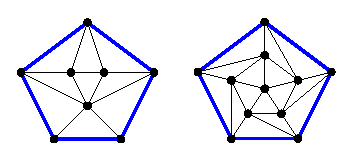
\includegraphics[width=0.9\textwidth]{images/example5.eps}
    \end{figure}
\end{frame}

\begin{frame}
    \frametitle{Example of non-reducible configurations on $R_5$.}
    \begin{figure}
        \centering
        \includegraphics[width=0.4\textwidth]{images/example5_bad.eps}
        \caption{Replacing this configuration by our reducer yields the same graph. Therefore, this configuration does not fall under the 1-reducibility of $R_5$. If it were, then the four color theorem would proven. }
    \end{figure}
\end{frame}
\begin{frame}
    \includegraphics[width=\textwidth]{images/break2.jpg}
    We will be back in 5 minutes.
\end{frame}

\section{Part 3}
\section{D-Reducibility}
\label{sec:dreduce}

We have seen that the ring $R_4$ is 0-reducible and the that the ring $R_5$ is 1-reducible. This essentially provides us with an two infinite classes of reducible configurations. However, it is not yet guaranteed that every planar graph contains such a $k$-reducible configuration on $R_4$ or $R_5$. Therefore, we must still look for more reducible configurations.

Naturally, we might try to examine the $k$-reducibility of $R_6$ and beyond. However, as we have seen in the increase in complexity for the 1-reducibility of $R_5$, this is a very tough problem. There are much more cases to consider for the ring $R_6$ than for $R_4$ and $R_5$. However, the difficulty of $k$-reducibility lies in the fact the we try to prove the reducibility of \textit{all} configurations $\confg$ on $R_n$ at once. Individual configurations are much easier to examine. 

Let us introduce the idea of D-reducibility, by working with an example. The very first, smallest and most famous configuration used in the proof of the four color theorem is the \textit{Birkhoff Diamond}  ($\text{Bir}\Diamond$). It is a configuration on $R_6$ with 4 vertices in the core.

\begin{figure}[!ht]
    \centering
    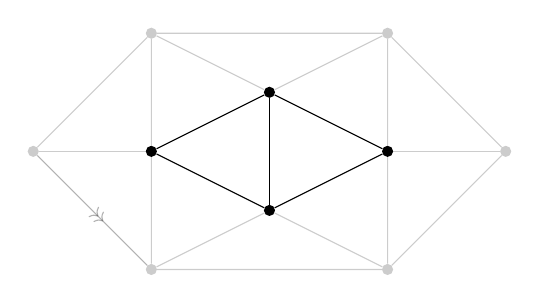
\begin{tikzpicture}[scale=1.5, mid arrow/.style={
        postaction={ decorate, decoration={ markings, mark=at position 0.6 with { \arrow[black]{>>} } } } }]
        \node[circle, fill, scale=0.015cm, opacity=0.2] (l1) at (-2, 0) { };
        \node[circle, fill, scale=0.015cm, opacity=0.2] (l2) at (-1, 1) { };
        \node[circle, fill, scale=0.015cm] (l3) at (-1, 0) {};
        \node[circle, fill, scale=0.015cm, opacity=0.2] (l4) at (-1, -1) {};

        \node[circle, fill, scale=0.015cm, opacity=0.2] (r1) at (2, 0) {};
        \node[circle, fill, scale=0.015cm, opacity=0.2] (r2) at (1, 1) {};
        \node[circle, fill, scale=0.015cm] (r3) at (1, 0) {};
        \node[circle, fill, scale=0.015cm, opacity=0.2] (r4) at (1, -1) {};

        \node[circle, fill, scale=0.015cm] (c1) at (0, 0.5) {};
        \node[circle, fill, scale=0.015cm] (c2) at (0, -0.5) {};

        \draw[opacity=0.2] (l1) -- (l2) -- (r2) -- (r1) -- (r4) -- (l4);
        \draw [mid arrow, opacity=0.3] (l1) -- (l4);
        \draw[opacity=0.2] (l1) -- (l3);
        \draw[opacity=0.2] (l2) -- (l3) -- (l4);
        \draw[opacity=0.2] (l2) -- (c1);
        \draw (c1) -- (l3) -- (c2);
        \draw[opacity=0.2] (c2) -- (l4);
        \draw (c1) -- (c2);
        \draw[opacity=0.2] (r2) -- (c1);
        \draw (c1) -- (r3) -- (c2);
        \draw[opacity=0.2] (c2) -- (r4);
        \draw[opacity=0.2] (r2) -- (r3) -- (r4);
        \draw[opacity=0.2] (r1) -- (r3);
    \end{tikzpicture}
    \caption{The Birkhoff Diamond $\confg = \bir$ with the core highlighted. }
    \label{fig:diamond}
\end{figure}

We highlighted the core $\core$ of the Birkhoff Diamond here, to explain the format of the \textit{unavoidable set of reducible configurations} found in the original proofs. Every (triangular) configuration with a ring is uniquely determined by its core $\core$ and the amount of edges that a vertex of the core $\core$ has in $\confg$.

For example, the Birkhoff Diamond is uniquely determined by the four vertices in the middle and the requirement that $\deg_\confg(v) = 5$ for each vertex in the core. To save space when storing configuations on paper or digitally, only this information of the core is actually needed.

We will show that $\bir$ is 0-reducible. Since we know the graph of $\bir$, we can write down all the colorings it can have on the ring. This is the set $\Phi(\bir)$ of 16 colorings. See Figure \ref{table:diamondphi0}.

\needspace{2cm}
\begin{figure}[!ht]
    \centering
    \begin{tabular}{ cccc }
        $\Phi(\bir) $ & \\
        \hline
        ababac & abacdb & abcadb & abcbcd \\
        ababcb & abacdc & abcbab & abcdab \\ 
        abacac & abcacb & abcbac & abcdcb \\
        abacbc & abcacd & abcbad & abcdcd \\
        \hline
        16 & \\
    \end{tabular}
    \caption{The unique ring colorings of $\bir$.}
    \label{table:diamondphi0}
\end{figure}

\needspace{1cm}
Therefore, if we want that $\bir$ is 0-reducible, we must show that any ring coloring of $M+R_6$ falls in the set $\Phi(\bir)$. When we were working with rings, we could only use the set of \textit{guaranteed} colorings of $\confg$. However, with an actual configuration like $\bir$, we know exactly which colorings are present. So we have much more control and precision to prove 0-reducibility.

If we let $M+R_6$ be arbitrary, then we can expect any ring coloring of $R_6$. Thus we must show that every coloring of $\Phi(6)$ can be changed to a coloring of $\Phi(\bir)$. The set $\Phi(6)$ can be seen in Figure \ref{table:colsring6}.

\begin{figure}[!ht]
    \centering
    \begin{tabular}{ cccc }
        $\Phi(6) $ & \\
        \hline
        ababab & abacbd & abcadc &  \cellcolor{g0} abcdab \\
        \cellcolor{g0} ababac &  \cellcolor{g0} abacdb &  \cellcolor{g0} abcbab & abcdac \\
        \cellcolor{g0} ababcb &  \cellcolor{g0} abacdc &  \cellcolor{g0} abcbac & abcdad \\
        ababcd & abcabc &  \cellcolor{g0} abcbad & abcdbc \\
        abacab & abcabd & abcbcb & abcdbd \\
        \cellcolor{g0} abacac &  \cellcolor{g0} abcacb &  \cellcolor{g0} abcbcd &  \cellcolor{g0} abcdcb \\
        abacad &  \cellcolor{g0} abcacd & abcbdb &  \cellcolor{g0} abcdcd \\
        \cellcolor{g0} abacbc &  \cellcolor{g0} abcadb & abcbdc \\
        \hline
        31 & \\
    \end{tabular}
    \caption{All unique ring colorings of $R_6$. The colorings of $\Phi(\bir)$ are highlighted. }
    \label{table:colsring6}
\end{figure}

As you can see, roughly half of the colorings is not directly compatible with $\bir$. Similar to what we did for the 1-reducibility of $R_5$, we will use Kempe-chains to change incompatible colorings to colorings in $\Phi(\bir)$.

Let us consider the coloring $ababab$ for example. Suppose that $\chain{v_4}{v_6}{bd}$. This implies the following colorings.

\begin{equation}
    \begin{aligned}
    \scheme{a,b,a,b,a,b}{46d} &\compat ababcb\\
    \scheme{a,b,a,b,a,b}{46d-} &\compat ababad = ababac.
    \end{aligned}
\end{equation}

Therefore, the coloring $ababab$ can be turned into a compatible coloring with only one chain flip. We say that the coloring $ababab$ \textit{implies} the set of colorings 

\begin{equation}
    ababab \compat \{ ababcb, ababac \}.
\end{equation}

This idea of a coloring implying a set of other colorings lies at the heart of D-reducibility, hence we will define it.

\begin{definition}
    A coloring $x$ implies a set of colorings $\II$ if every scheme $x^\star$ of $x$ implies a coloring $y \in \II$. Write $x \compat \II$.
\end{definition}

\begin{definition}
    A set of colorings $\I$ implies $\II$ if every $x \in \I$ implies $\II$. Write $\I \implies \II$.
\end{definition}

Now, let us find all the colorings of $R_6$ that require one chain flip to become compatible in the same way as $ababab$. This set is called the 1-implying set of $\bir$.

\begin{figure}[!ht]
    \centering
    \begin{tabular}{ cc }
        $\Phi_1(\bir) $ \\
        \hline
        ababab & abcbcb \\
        ababcd & abcdad\\
        abacab \\
        \hline
        5 \\
    \end{tabular}
    \caption{The 1-implying set $\Phi_1(\bir)$.}
    \label{table:diamondphi1}
\end{figure}

This is the largest set that satisfies $\Phi_1(\bir) \compat \Phi(\bir)$. We may repeat what we did for $\Phi_1(\bir)$ to obtain sets of colorings that require 2, 3 and more chain flips to become a coloring in $\Phi(\bir)$.

\begin{equation}
    \Phi_5(\bir) \compat \Phi_4(\bir) \compat \Phi_3(\bir) \compat \ldots \compat \Phi(\bir).
\end{equation}

Let us first define the notion of higher-order implication between sets of colorings, called \textit{n-implication}.

\begin{definition}
    A set of colorings $\I$ $n$-implies a set $\II$ if there exist sets $B_i$ for $0 < i < n$ such that $I \compat B_{n-1}$, $B_i \compat B_{i-1}$ and $B_1 \compat \II$. We write $\I \ncompat{n} \II$.
\end{definition}

Therefore the set $\Phi_5(\bir)$, for example, satisfies $\Phi_5(\bir) \ncompat{5} \Phi_0(\bir)$. This is essentially the definition of the $n$-implying set of $\bir$.

\begin{definition}
    The $n$-implying set $\Phi_n(\confg)$ of a configuration $\confg$ is the largest set of ring colorings such that $\Phi_n(C) \ncompat{n} \Phi_0(\confg) = \Phi(\confg)$. 
\end{definition}

To continue with our example, let us find all the $n$-implying sets of $\bir$. In this case, there are only 6 including $\Phi_0(\bir)$.

\needspace{2cm}
\begin{figure}[!ht]
    \centering
    \begin{tabular}{ ccccccc }
        $\Phi_0(\bir) $ & & $\Phi_1$ & $\Phi_2$ & $\Phi_3$ & $\Phi_4$ & $\Phi_5$ \\
        \hline
        ababac & abcadb & ababab & abacad & abacbd & abcabd & abcabc \\
        ababcb & abcbab & ababcd & abcbdb & abcbdc & abcadc & \\
        abacac & abcbac & abacab &        & abcdac & abcdbc & \\
        abacbc & abcbad & abcbcb &        & abcdbd &        & \\
        abacdb & abcbcd & abcdad &        &        &        & \\
        abacdc & abcdab \\
        abcacb & abcdcb \\
        abcacd & abcdcd \\
        \hline
        16 & & 5 & 2 & 4 & 3 & 1 \\
    \end{tabular}
    \caption{ All $n$-implying sets of $\bir$. Together a total of 31 colorings. }
    \label{table:diamondmap}
\end{figure}

If you count the colorings, you will find that all $n$-implying sets together form 31 colorings. This is exactly the number of ring colorings of $R_6$. Therefore, all colorings of $R_6$ can be made compatible with $\bir$ through chain flips. This is exactly what D-reducibility requires.

\begin{definition}
    The \emph{max-implying} set $\overline{\Phi}(\confg)$ of a configuration $\confg$ is the largest $n$-implying set  $\Phi_n(\confg)$.
\end{definition}

\begin{definition}
    A configuration $\confg$ on $R_n$ is D-reducible if $\overline{\Phi}(\confg) = \Phi(n)$.
\end{definition}

\begin{figure}[!h]
    \centering
    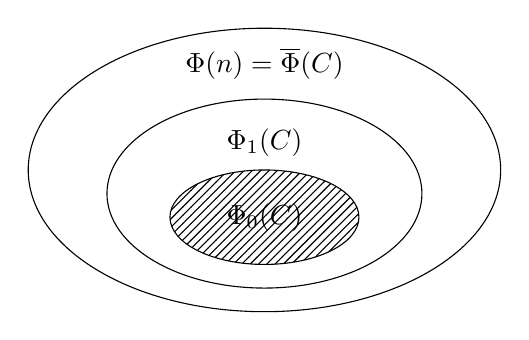
\begin{tikzpicture}[scale=1.0]
        \draw (0, 0) ellipse (3cm and 1.8cm);
        \draw (0, -0.3) ellipse (2cm and 1.2cm);
        \draw[fill opacity=0.4, pattern=north east lines] (0, -0.6) ellipse (1.2cm and 0.6cm);

        \node at (0.0, -0.6) { $\Phi_0(C)$ };
        \node at (0.0, 0.35) { $\Phi_1(C)$ };
        \node at (0, 1.35) { $\Phi(n) = \overline{\Phi}(C)$ };
    \end{tikzpicture}

    \caption{The $n$-implying sets of $\confg$ are increasing in size. If they grow to the set of all ring colorings $\Phi(n)$, the configuration is D-reducible. }
\end{figure}

However, it can occur that $\overline{\Phi}(\confg) \neq \Phi(n)$. This is the case with the ring $R_5$ with a single vertex on the inside, which only supports 3-colorings. To handle (some) of these configurations, a stronger form of D-reducibility was required. This is where we go to C-reducibility.
\subsection{C-reducibility}
\begin{frame}
    \frametitle{The Bernhart Diamond}

    \begin{figure}[!h]
        \centering
        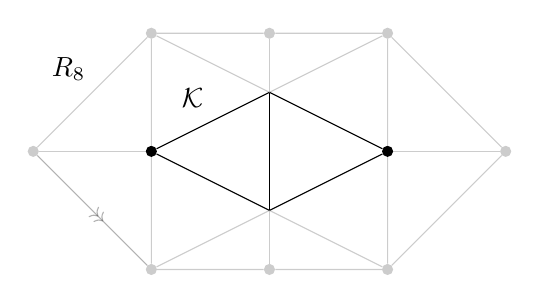
\begin{tikzpicture}[scale=1.5, mid arrow/.style={
            postaction={ decorate, decoration={ markings, mark=at position 0.6 with { \arrow[black]{>>} } } } }]
            \node[circle, fill, scale=0.015cm, opacity=0.2] (l1) at (-2, 0) { };
            \node[circle, fill, scale=0.015cm, opacity=0.2] (l2) at (-1, 1) { };
            \node[circle, fill, scale=0.015cm] (l3) at (-1, 0) {};
            \node[circle, fill, scale=0.015cm, opacity=0.2] (l4) at (-1, -1) {};
    
            \node[circle, fill, scale=0.015cm, opacity=0.2] (r1) at (2, 0) {};
            \node[circle, fill, scale=0.015cm, opacity=0.2] (r2) at (1, 1) {};
            \node[circle, fill, scale=0.015cm] (r3) at (1, 0) {};
            \node[circle, fill, scale=0.015cm, opacity=0.2] (r4) at (1, -1) {};
    
            \node[circle, fill, scale=0.001cm] (c1) at (0, 0.5) {};
            \node[circle, fill, scale=0.001cm] (c2) at (0, -0.5) {};
            \node[circle, fill, scale=0.015cm, opacity=0.2] (b1) at (0, 1) {};
            \node[circle, fill, scale=0.015cm, opacity=0.2] (b2) at (0, -1) {};
            \node (core) at (-0.65, 0.45) { $\core$ };
            \node (ring) at (-1.7, 0.7) { $R_8$ };
    
            \draw[opacity=0.2] (l1) -- (l2) -- (b1) -- (r2) -- (r1) -- (r4) -- (b2) -- (l4);
            \draw[opacity=0.2] (c1) -- (b1);
            \draw[opacity=0.2] (c2) -- (b2);
    
            \draw [mid arrow, opacity=0.3] (l1) -- (l4);
            \draw[opacity=0.2] (l1) -- (l3);
            \draw[opacity=0.2] (l2) -- (l3) -- (l4);
            \draw[opacity=0.2] (l2) -- (c1);
            \draw (c1) -- (l3) -- (c2);
            \draw[opacity=0.2] (c2) -- (l4);
            \draw (c1) -- (c2);
            \draw[opacity=0.2] (r2) -- (c1);
            \draw (c1) -- (r3) -- (c2);
            \draw[opacity=0.2] (c2) -- (r4);
            \draw[opacity=0.2] (r2) -- (r3) -- (r4);
            \draw[opacity=0.2] (r1) -- (r3);
        \end{tikzpicture}
        \caption{The Bernhart Diamond ($\ber$). An example of a non D-reducible configuration. Why? }
    \end{figure}
    
\end{frame}

\begin{frame}
    \frametitle{C-reducibility}

    \begin{itemize}
        \item \colorbox{g0}{\underline{valid}} 
        \item \colorbox{g0}{fixable} 
        \item \colorbox{rg}{reducer fixable}
        \item \colorbox{rb}{reducer unfixable}
        \item \colorbox{sf}{\textcolor{white}{symmetry fault}}
        \item unfixable
    \end{itemize}
    \begin{figure}
        \begin{tikzpicture}[overlay]
            \node at (3.5,2.5) {\includegraphics[height=9.3cm]{images/bigass.pdf}};
        \end{tikzpicture}
    \end{figure}
\end{frame}

\begin{frame}
    \frametitle{Reducers again}

    Reducers can be used to restrict the possible ring colorings. We need a reducer whose generated colorings are all \colorbox{g0}{fixable}. We have already seen reducers when proving the 1-reducibility of $R_5$!

    A reducer consists of a contraction and  extra interior edges and vertices.
    \begin{figure}[!h]
        \centering
        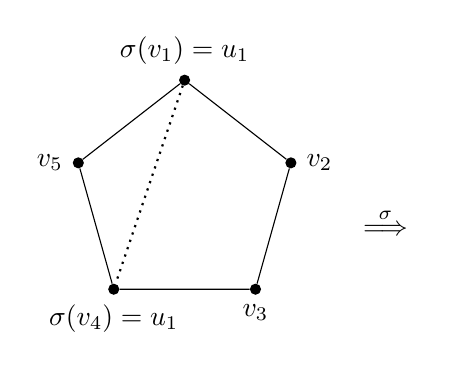
\begin{tikzpicture}[scale=1.5]
            \node[circle, fill, scale=0.015cm, label=above:{$\sigma(v_1)= u_1$}] (l1) at (0, 1) { };
            \node[circle, fill, scale=0.015cm, label=right:{$v_2$}] (l2) at (0.9, 0.30) { };
            \node[circle, fill, scale=0.015cm, label=below:{$v_3$}] (l3) at (0.6, -0.77) {};
            \node[circle, fill, scale=0.015cm, label=below:{$\sigma(v_4)=u_1$}] (l4) at (-0.6, -0.77) {};
            \node[circle, fill, scale=0.015cm, label=left:{$v_5$}] (l5) at (-0.9, 0.30) {};
            \draw (l1) -- (l2) -- (l3) -- (l4) -- (l5) -- (l1);
            \draw[dotted, thick] (l1) -- (l4);
            \node at (1.7, -0.2) { $\stackrel{\sigma}{\implies}$ };
        \end{tikzpicture}
        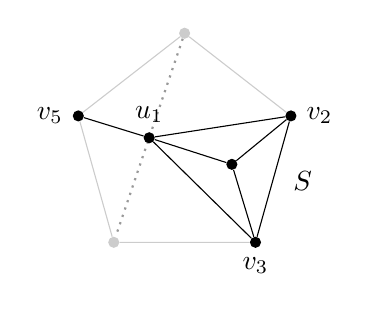
\begin{tikzpicture}[scale=1.5]
            \node[circle, fill, opacity=0.2, scale=0.015cm] (l1) at (0, 1) {};
            \node[circle, fill, opacity=0.2, scale=0.015cm] (l4) at (-0.6, -0.77) {};
            \node[circle, fill, scale=0.015cm, label=above:{$u_1$}] (y1) at (-0.3, 0.115) {};
    
            \node[circle, fill, scale=0.015cm, label=right:{$v_2$}] (l2) at (0.9, 0.30) { };
            \node[circle, fill, scale=0.015cm, label=below:{$v_3$}] (l3) at (0.6, -0.77) {};
            \node[circle, fill, scale=0.015cm, label=left:{$v_5$}] (l5) at (-0.9, 0.30) {};
    
            \node[circle, fill, scale=0.015cm] (s) at (0.4, -0.11) { };
            \node (s1) at (1.0, -0.25) { $S$ };
    
            \draw (s) -- (y1);
            \draw (s) -- (l3);
            \draw (s) -- (l2);

            \draw (l5) -- (y1) -- (l2) -- (l3) -- (y1);
            \draw[dotted, thick, opacity=0.4] (l1) -- (l4);
            \draw[opacity=0.2] (l5) -- (l1) -- (l2);
            \draw[opacity=0.2] (l3) -- (l4) -- (l5);
        \end{tikzpicture}
    \end{figure}
\end{frame}

\begin{frame}
    \frametitle{Reducers again}

    \begin{definition}
        A ring contraction $\sigma(v)$ on $R$ is a map from $R$ to the contracted ring $\sigma(R)$. Neighboring vertices of $R$ may not be mapped to the same vertex by $\sigma$.
    \end{definition}
    
    \begin{figure}[!h]
        \centering
        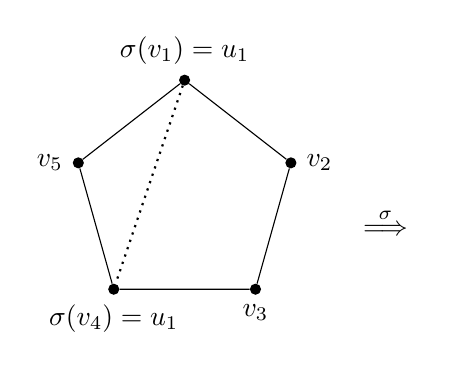
\begin{tikzpicture}[scale=1.5]
            \node[circle, fill, scale=0.015cm, label=above:{$\sigma(v_1)= u_1$}] (l1) at (0, 1) { };
            \node[circle, fill, scale=0.015cm, label=right:{$v_2$}] (l2) at (0.9, 0.30) { };
            \node[circle, fill, scale=0.015cm, label=below:{$v_3$}] (l3) at (0.6, -0.77) {};
            \node[circle, fill, scale=0.015cm, label=below:{$\sigma(v_4)=u_1$}] (l4) at (-0.6, -0.77) {};
            \node[circle, fill, scale=0.015cm, label=left:{$v_5$}] (l5) at (-0.9, 0.30) {};
            \draw (l1) -- (l2) -- (l3) -- (l4) -- (l5) -- (l1);
            \draw[dotted, thick] (l1) -- (l4);
            \node at (1.7, -0.2) { $\stackrel{\sigma}{\implies}$ };
        \end{tikzpicture}
        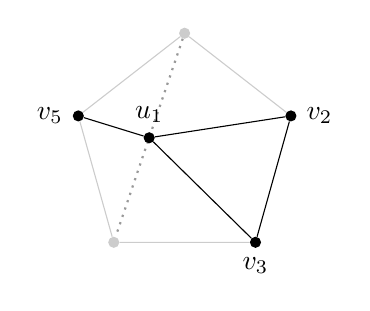
\begin{tikzpicture}[scale=1.5]
            \node[circle, fill, opacity=0.2, scale=0.015cm] (l1) at (0, 1) {};
            \node[circle, fill, opacity=0.2, scale=0.015cm] (l4) at (-0.6, -0.77) {};
            \node[circle, fill, scale=0.015cm, label=above:{$u_1$}] (y1) at (-0.3, 0.115) {};
    
            \node[circle, fill, scale=0.015cm, label=right:{$v_2$}] (l2) at (0.9, 0.30) { };
            \node[circle, fill, scale=0.015cm, label=below:{$v_3$}] (l3) at (0.6, -0.77) {};
            \node[circle, fill, scale=0.015cm, label=left:{$v_5$}] (l5) at (-0.9, 0.30) {};

            \draw (l5) -- (y1) -- (l2) -- (l3) -- (y1);
            \draw[dotted, thick, opacity=0.4] (l1) -- (l4);
            \draw[opacity=0.2] (l5) -- (l1) -- (l2);
            \draw[opacity=0.2] (l3) -- (l4) -- (l5);
        \end{tikzpicture}
    \end{figure}
    
\end{frame}

\begin{frame}
    \frametitle{Reducers again}

    \begin{definition}
        A reducer $(S,\sigma)$ of a configuration $\confg$ consists of
        \begin{itemize}
            \item A contraction $\sigma(v)$ on $R$.
            \item A graph $|S| < |\confg|$ whose boundary is the contracted ring $\sigma(R)$.
        \end{itemize}
    \end{definition}
    
    \begin{figure}[!h]
        \centering
        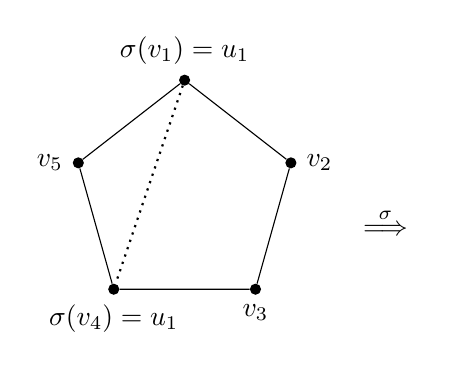
\begin{tikzpicture}[scale=1.5]
            \node[circle, fill, scale=0.015cm, label=above:{$\sigma(v_1)= u_1$}] (l1) at (0, 1) { };
            \node[circle, fill, scale=0.015cm, label=right:{$v_2$}] (l2) at (0.9, 0.30) { };
            \node[circle, fill, scale=0.015cm, label=below:{$v_3$}] (l3) at (0.6, -0.77) {};
            \node[circle, fill, scale=0.015cm, label=below:{$\sigma(v_4)=u_1$}] (l4) at (-0.6, -0.77) {};
            \node[circle, fill, scale=0.015cm, label=left:{$v_5$}] (l5) at (-0.9, 0.30) {};
            \draw (l1) -- (l2) -- (l3) -- (l4) -- (l5) -- (l1);
            \draw[dotted, thick] (l1) -- (l4);
            \node at (1.7, -0.2) { $\stackrel{\sigma}{\implies}$ };
        \end{tikzpicture}
        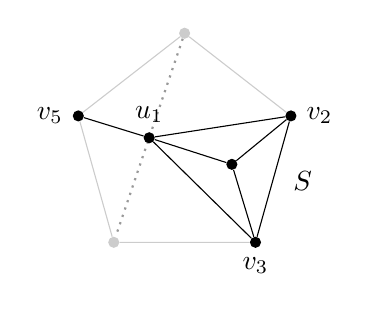
\begin{tikzpicture}[scale=1.5]
            \node[circle, fill, opacity=0.2, scale=0.015cm] (l1) at (0, 1) {};
            \node[circle, fill, opacity=0.2, scale=0.015cm] (l4) at (-0.6, -0.77) {};
            \node[circle, fill, scale=0.015cm, label=above:{$u_1$}] (y1) at (-0.3, 0.115) {};
    
            \node[circle, fill, scale=0.015cm, label=right:{$v_2$}] (l2) at (0.9, 0.30) { };
            \node[circle, fill, scale=0.015cm, label=below:{$v_3$}] (l3) at (0.6, -0.77) {};
            \node[circle, fill, scale=0.015cm, label=left:{$v_5$}] (l5) at (-0.9, 0.30) {};
            \node[circle, fill, scale=0.015cm] (s) at (0.4, -0.11) { };
            \node (s1) at (1.0, -0.25) { $S$ };
    
            \draw (s) -- (y1);
            \draw (s) -- (l3);
            \draw (s) -- (l2);
            \draw (l5) -- (y1) -- (l2) -- (l3) -- (y1);
            \draw[dotted, thick, opacity=0.4] (l1) -- (l4);
            \draw[opacity=0.2] (l5) -- (l1) -- (l2);
            \draw[opacity=0.2] (l3) -- (l4) -- (l5);
        \end{tikzpicture}
    \end{figure}
    
\end{frame}

\begin{frame}
    \frametitle{Reducer for the Bernhart Diamond}

    \begin{figure}[!h]
        \centering
        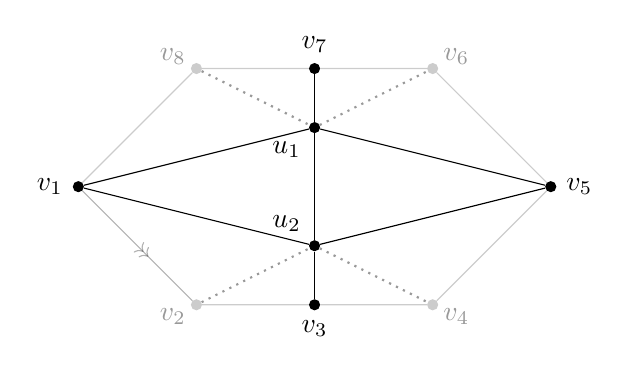
\begin{tikzpicture}[scale=1.5, mid arrow/.style={
            postaction={ decorate, decoration={ markings, mark=at position 0.6 with { \arrow[black]{>>} } } } }]
            \node[circle, fill, scale=0.015cm, label=left:$v_1$] (l1) at (-2, 0) { };
            \node[opacity=0.4] at (-1.2, 1.1) { $v_8$ };
            \node[circle, fill, scale=0.015cm, opacity=0.2] (l2) at (-1, 1) { };
            \node[opacity=0.4] at (-1.2, -1.1) { $v_2$ };
            \node[circle, fill, scale=0.015cm, opacity=0.2] (l4) at (-1, -1) {};
    
            \node[circle, fill, scale=0.015cm, label=right:$v_5$] (r1) at (2, 0) {};
            \node[opacity=0.4] at (1.2, 1.1) { $v_6$ };
            \node[circle, fill, scale=0.015cm, opacity=0.2] (r2) at (1, 1) {};
            \node[opacity=0.4] at (1.2, -1.1) { $v_4$ };
            \node[circle, fill, scale=0.015cm, opacity=0.2] (r4) at (1, -1) {};
    
            \node[circle, fill, scale=0.015cm, label=above:$v_7$] (b1) at (0, 1) {};
            \node[circle, fill, scale=0.015cm, label=below:$v_3$] (b2) at (0, -1) {};
            \node[circle, fill, scale=0.015cm, label=below left:$u_1$] (u1) at (0, 0.5) {};
            \node[circle, fill, scale=0.015cm, label=above left:$u_2$] (u2) at (0, -0.5) {};
    
            \draw[opacity=0.2] (l1) -- (l2) -- (b1) -- (r2) -- (r1) -- (r4) -- (b2) -- (l4);
            \draw [mid arrow, opacity=0.3] (l1) -- (l4);
            \draw (l1) -- (u1) -- (r1) -- (u2) -- (l1);
            \draw (b1) -- (u1);
            \draw (b2) -- (u2);
            \draw (u1) -- (u2);
            \draw[dotted, thick, opacity=0.4] (l2) -- (u1) -- (r2);
            \draw[dotted, thick, opacity=0.4] (l4) -- (u2) -- (r4);
    
        \end{tikzpicture}
    \end{figure}

    The reducer generates the following type of colorings.
    \begin{equation}
        v_1\;\colorbox{cyan}{$u_2$}\;v_3\;v_5\;\colorbox{magenta}{$u_1$}\;v_7 \quad \mapsto \quad v_1\;\colorbox{cyan}{$u_2$}\;v_3\;\colorbox{cyan}{$u_2$}\;v_5\;\colorbox{magenta}{$u_1$}\;v_7\;\colorbox{magenta}{$u_1$}.
    \end{equation}
\end{frame}

\begin{frame}
    \frametitle{C-reducibility}

    \begin{definition}
        A configuration $\confg$ is C-reducible if $\Phi(S,\sigma) \subset \overline{\Phi}(\confg)$ for some reducer $(S,\sigma)$.
    \end{definition}

    \begin{example}
        The Bernhart Diamond $(\ber)$ is C-reducible. The red colorings are \textit{symmetry faults} that can be shown to be fixable
    \end{example}
\end{frame}

\begin{frame}
    \frametitle{Symmetry Faults}

    The two red colorings generated by the reducer are not fixable. Does this mean that $\ber$ is not C-reducible?

    \begin{equation}
        \begin{aligned}
            \colorbox{rb}{abcbacbc} &\quad (R1) \\ \quad \colorbox{rb}{abcbdcbc} &\quad (R2)
        \end{aligned}
    \end{equation}

    \uncover<2->{
        Bernhart has shown in 1947 that these colorings \textit{can} in fact be fixed. So there must be an error in $\maxi{\ber}$.
    }
\end{frame}


\begin{frame}
    \frametitle{Symmetry Faults}

    Consider the following colorings.

    \begin{equation}
        \begin{aligned}
            \colorbox{rb}{abcbacbc} &\quad (R1) & \colorbox{sf}{\textcolor{white}{abcbadbc}} &\quad (F1) & \colorbox{rg}{\underline{abcbacac}} &\quad (G1)\\
             \quad \colorbox{rb}{abcbdcbc} &\quad (R2) & \quad \colorbox{g0}{abcbacbd} &\quad (F1\star) & \quad \colorbox{g0}{\underline{abcbdbcb}} &\quad (G2) \\
        \end{aligned}
    \end{equation}

    \uncover<2->{
    Then we have the implications

    \begin{equation}
        \begin{aligned}
        R2 \compat \{ G2, &R1 \} \\
        &\downarrow \\
        &R1 \compat \{ G1, F1 \} \\
        \end{aligned}
    \end{equation}

    Therefore, fixability of $R1$ and $R2$ depends fully on $F1$.
    }
\end{frame}

\begin{frame}
    \frametitle{Symmetry Faults}

    \begin{equation}
        \begin{aligned}
            \colorbox{rb}{abcbacbc} &\quad (R1) & \colorbox{sf}{\textcolor{white}{abcbadbc}} &\quad (F1) & \colorbox{rg}{\underline{abcbacac}} &\quad (G1)\\
             \quad \colorbox{rb}{abcbdcbc} &\quad (R2) & \quad \colorbox{g0}{abcbacbd} &\quad (F1\star) & \quad \colorbox{g0}{\underline{abcbdbcb}} &\quad (G2) \\
        \end{aligned}
    \end{equation}

    \begin{figure}[!h]
        \centering
        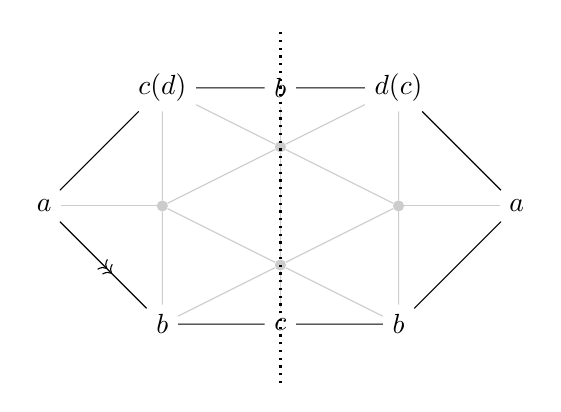
\begin{tikzpicture}[scale=1.5, mid arrow/.style={
            postaction={ decorate, decoration={ markings, mark=at position 0.6 with { \arrow[black]{>>} } } } }]
            \node (l1) at (-2, 0) { $a$ };
            \node (l2) at (-1, 1) { $c(d)$ };
            \node[circle, fill, scale=0.015cm, opacity=0.2] (l3) at (-1, 0) {};
            \node (l4) at (-1, -1) { $b$ };
    
            \node (r1) at (2, 0) { $a$ };
            \node (r2) at (1, 1) { $d(c)$ };
            \node[circle, fill, scale=0.015cm, opacity=0.2] (r3) at (1, 0) {};
            \node (r4) at (1, -1) { $b$ };
    
            \node[circle, fill, scale=0.015cm, opacity=0.2] (c1) at (0, 0.5) {};
            \node[circle, fill, scale=0.015cm, opacity=0.2] (c2) at (0, -0.5) {};
            \node (b1) at (0, 1) { $b$ };
            \node (b2) at (0, -1) { $c$ };
    
            \draw[thick, dotted] (0, -1.5) -- (0, 1.5);
            \draw[opacity=1.0] (l1) -- (l2) -- (b1) -- (r2) -- (r1) -- (r4) -- (b2) -- (l4);
            \draw[opacity=0.2] (c1) -- (b1);
            \draw[opacity=0.2] (c2) -- (b2);
    
            \draw [mid arrow, opacity=1.0] (l1) -- (l4);
            \draw[opacity=0.2] (l1) -- (l3);
            \draw[opacity=0.2] (l2) -- (l3) -- (l4);
            \draw[opacity=0.2] (l2) -- (c1);
            \draw[opacity=0.2] (c1) -- (l3) -- (c2);
            \draw[opacity=0.2] (c2) -- (l4);
            \draw[opacity=0.2] (c1) -- (c2);
            \draw[opacity=0.2] (r2) -- (c1);
            \draw[opacity=0.2] (c1) -- (r3) -- (c2);
            \draw[opacity=0.2] (c2) -- (r4);
            \draw[opacity=0.2] (r2) -- (r3) -- (r4);
            \draw[opacity=0.2] (r1) -- (r3);
        \end{tikzpicture}
    \end{figure}

    \uncover<2->{
        The colorings $F1$ and $F1\star$ are symmetric. Therefore, $F1$ must be fixable!
    }
\end{frame}

\begin{frame}
    \begin{definition}<1->
        A graph symmetry of $G$ is a bijection $f(v)$ on the vertices of $G$ that preserves the neighbors of every vertex.
    \end{definition}
    
    \begin{definition}<2->
        A \emph{symmetry fault} of a configuration $\confg$ is a coloring $x$ that is not in $\maxi{\confg}$, but whose symmetry $x\star = f(x)$ is.
    \end{definition}

    \uncover<3->{
        Bernhart mentioned the same problematic colorings in his proof. Is it a coincidence? We have not delved deeper into this problem.
    }
\end{frame}
\section{Conclusion}
\begin{frame}
    \frametitle{Conclusion}
    \begin{itemize}
        \item $k$-reducibility extends upon ideas from the Five Color Theorem.
        \item D-reducibility extends upon $k$-reducibility for rings 6 and above.
        \item C-reducibility extends upon D-reducibility by avoiding bad ring colorings.
        \item Unavoidability guarantees that every planar graph has a reducible configuration.
        \item The Birkhoff Diamond and Bernhart Diamond illustrate D and C-reducibility.
        \item Symmetry faults in the Bernhart Diamond require more attention.
    \end{itemize}
\end{frame}

\begin{frame}
    \frametitle{Conclusion}

    The more advanced the concept of reducibility, the less reducible configurations are needed (A/B-reducibility is a case of C reducibility).

    \vspace{1cm}
    \begin{figure}
        \centering
        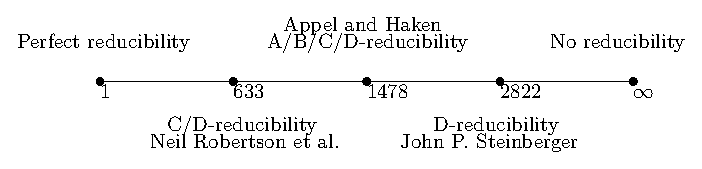
\includegraphics[width=1.0\textwidth]{images/reduce.eps}
        \caption{Number of reducible configurations on rings $R_6$ and higher in proofs of the four color theorem}.
    \end{figure}

    \uncover<2->{
        Does "Perfect reducibility" exist? If so, it will be the heart of the four color theorem.
    }
\end{frame}

\begin{frame}
    \frametitle{The End}
    Thank you for your attention. Questions?
\end{frame}

\end{document}